\documentclass[runningheads]{llncs}

\usepackage[review,year=2026,ID=00000]{eccv}
\usepackage{eccvabbrv}
\usepackage{graphicx}
\usepackage{booktabs}
\usepackage{url}
\usepackage[pagebackref,breaklinks,colorlinks,citecolor=eccvblue]{hyperref}

\begin{document}

\title{Joint Movie Context for Long-Video QA}
\titlerunning{Joint Movie Context for Long-Video QA}
\author{Anonymous ECCV 2026 Submission}
\authorrunning{Anonymous ECCV 2026 Submission}
\institute{Paper ID \#00000}
\maketitle

\begin{abstract}
This artifact describes a movie-level answer-bank pipeline for open-ended long-video question answering. The system groups questions from one film, exposes shared timestamped and visual evidence, and emits one validated JSON answer bank. Videos, labels, generated answers, credentials, and submission records remain external inputs.
\keywords{long-video understanding \and movie question answering \and reproducibility \and anonymous artifact}
\end{abstract}

\section{Task and Artifact Boundary}

The task is open-ended question answering over short films. Questions may
require an early name, a changing relation, or the final state of an event
chain. The movie is the context unit. The release contains source code, tests,
and documentation only; data, videos, weights, answers, credentials, account
identifiers, leaderboard records, and absolute paths remain external
inputs~\cite{sf20kdata2026,slomo2026}.

\section{Movie-Level Inference Contract}

For each movie $m$, the runner constructs one request:
\begin{equation}
  (E_m,Q_m) \longrightarrow \{a_{m,1},a_{m,2},\ldots,a_{m,n_m}\},
\end{equation}
where $E_m$ is shared evidence and $Q_m$ is the complete question set. The
model returns one JSON object keyed by the original question IDs.

The prompt requires consistent names, aliases, relationships, event order,
causes, repeated objects, and ending state. Frames are chronological JPEGs with
timestamp markers; long transcripts use a head-and-tail bound.

\begin{center}
  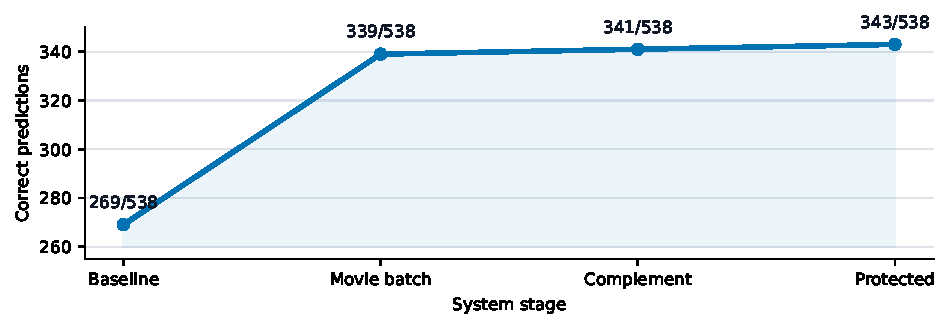
\includegraphics[width=.68\linewidth]{figures/official_progress.pdf}
  \captionof{figure}{Historical official score chain. The discontinuity appears at the movie-batched multimodal source; later parent-preserving changes are smaller. Values are correct predictions out of 538.}
  \label{fig:progress}
\end{center}

\newpage

\section{Validation and Failure Handling}

The runner reads credentials only from a process environment variable. A movie
result is persisted only after the response parses as JSON and contains every
requested question ID with a non-empty answer. Partial movie responses are
never silently merged with another protocol.

The conversion and audit scripts enforce this upload contract~\cite{evalai2026}:
\begin{itemize}
  \item exact header: \texttt{question\_id,prediction};
  \item every required question ID appears exactly once;
  \item all predictions are non-empty;
  \item public and private annotations remain separate;
  \item inference does not read answer keys, options, private labels, or
        leaderboard output.
\end{itemize}

\section{Evidence-Bound Diagnostics}

The plots are generated from \texttt{figures/figure\_data.json} by a
deterministic script. Figure~\ref{fig:factors} reports a frozen six-movie,
60-question factor audit: joint answering reaches 27/60, independent calls
18/60, no frames 24/60, Target16 29/60, and Dense48 30/60. The diagnostics
support joint context and bound claims about simple frame changes.

\begin{center}
  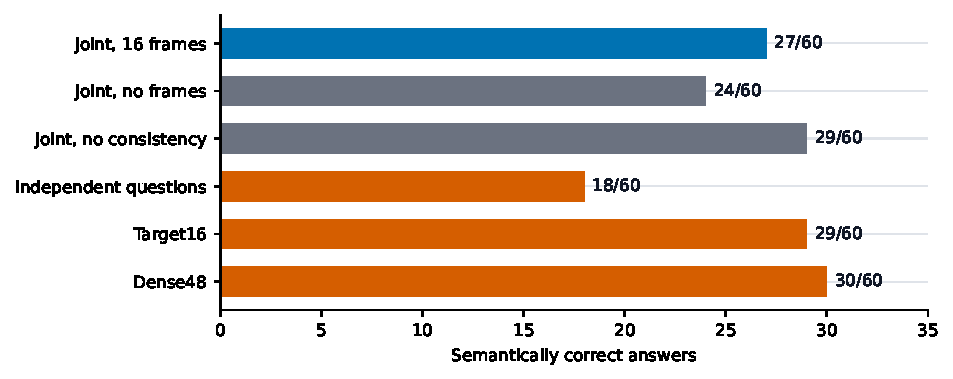
\includegraphics[width=.82\linewidth]{figures/factor_audit.pdf}
  \captionof{figure}{Frozen factor and visual-ceiling audit on six movies. Blue is the direct reference; orange bars are controlled variants. Scores are local diagnostics, not official leaderboard results.}
  \label{fig:factors}
\end{center}

\section{Reproducibility and Anonymous Submission}

The repository starts from a fresh Git history with anonymous author metadata.
The ECCV review template replaces author and affiliation fields with a paper-ID
placeholder and enables line numbering. Replace the placeholder only with the
assigned ID before submission; do not add author names or identifying links.

The live SLoMO page remains authoritative for deadlines, track rules, and
artifact policy~\cite{slomo2026}. Reproduction requires authorized data and
model access followed by the repository schema audit.

\clearpage

\bibliographystyle{splncs04}
\bibliography{technical_document_eccv}

\end{document}
